\documentclass[a4paper,12pt]{report}

\usepackage{graphicx}
\usepackage{amsmath}
\usepackage{fullpage}
\usepackage[parfill]{parskip}
\usepackage{amssymb}
\usepackage{alltt}

\newcommand{\degree}{\ensuremath{^\circ}}
\newcommand{\unit}[1]{\ensuremath{\, \mathrm{#1}}}

\begin{document}
\title{VirtualBox, Binary to Decimal Conversion and Networking Commands}
\author{Kimberley Manning}
\date{21 September 2012}
\newpage

\section*{COMP30040 - Assignment 1}

\subsubsection*{VirtualBox, Binary to Decimal Conversion and Networking Commands}

\textbf{Question 1}

Check that VirtualBox is installed:

\begin{verbatim}
[kimberley@promethei]$ rpm -qa | grep VirtualBox
VirtualBox-4.1.18-1.fc17.x86_64
kmod-VirtualBox-3.5.3-1.fc17.x86_64-4.1.18-1.fc17.7.x86_64
\end{verbatim}

After Ubuntu 12.04 LTS is installed on a new virtual machine:

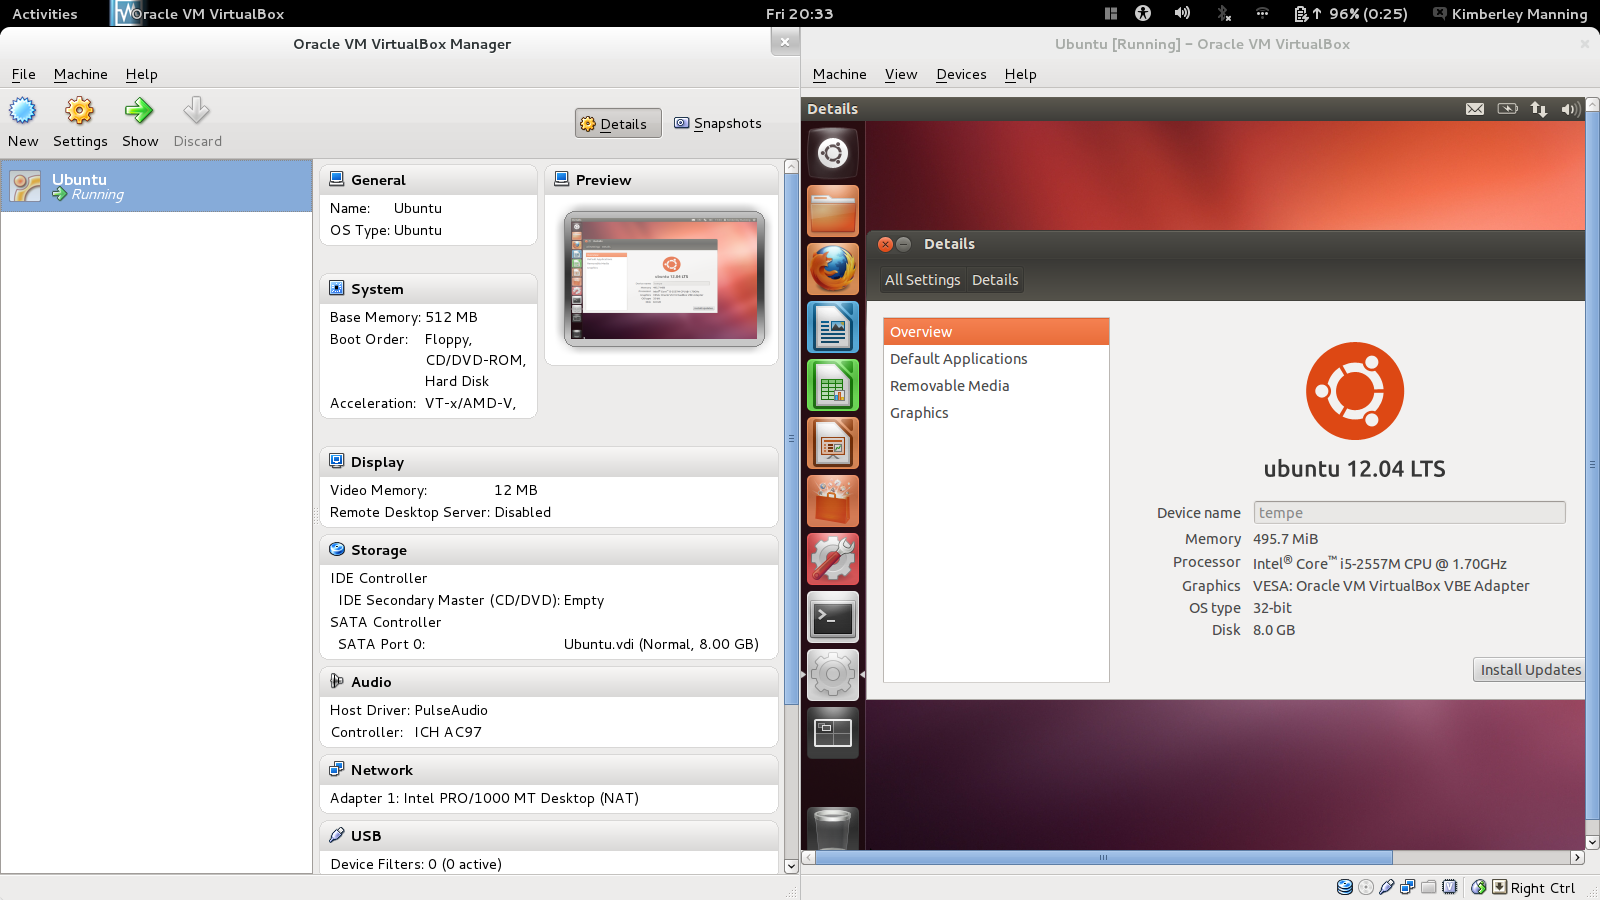
\includegraphics[width=\textwidth]{virtualbox-setup.png}

\textbf{Question 2}

a) Binary is a positional number system in base-2. The right-most digit represents $2^0$, the digit to its left $2^1$, and so on, and each binary digit (bit) can only take the value 0 or 1. Binary numbers can be converted to decimal by multiplying the value of each bit by the power of 2 matching its position, and summing the products. For example:

$10101010_2 = 1(2^7)+0(2^6)+1(2^5)+0(2^4)+1(2^3)+0(2^2)+1(2^1)+0(2^0) = 170_{10}$

$11110000_2 = 2^7+2^6+2^5+2^4 = 240_{10}$

$10100000_2 = 2^7+2^5 = 160_{10}$

$00001111_2 = 2^3+2^2+2^1+2^0 = 15_{10}$

IP addresses are sometimes represented in binary:

$00100111.11101110.01101001.00000100 = 39.238.105.4$

b) One method for converting decimal numbers to binary is by subtracting descending powers of two until the remainder is 0:

\begin{eqnarray*}
    255 &=& 2^7 + 127 \\
    127 &=& 2^6 + 63 \\
    63 &=& 2^5 + 31 \\
    31 &=& 2^4 + 15 \\
    15 &=& 2^3 + 7 \\
    7 &=& 2^2 + 3 \\
    3 &=& 2^1 + 1 \\
    1 &=& 2^0 + 0
\end{eqnarray*}

\begin{equation*}
    \therefore 255_{10} = 2^7 + 2^6 + 2^5 + 2^4 + 2^3 + 2^2 + 2^1 + 2^0 = 11111111_2
\end{equation*}

A similar method is repeated division by 2. Reading up the remainder column gives the number in binary:

\begin{eqnarray*}
    163 \div 2 &=& 81 \text{ r } 1 \\
    81 \div 2 &=& 40 \text{ r } 1 \\
    40 \div 2 &=& 20 \text{ r } 0 \\
    20 \div 2 &=& 10 \text{ r } 0 \\
    10 \div 2 &=& 5 \text{ r } 0 \\
    5 \div 2 &=& 2 \text{ r } 1 \\
    2 \div 2 &=& 1 \text{ r } 0 \\
    1 \div 2 &=& 0 \text{ r } 1
\end{eqnarray*}

\begin{equation*}
    \therefore 163_{10} = 10100011_2
\end{equation*}

Therefore:

$255_{10} = 11111111_2$

$254_{10} = 11111110_2$

$163_{10} = 10100011_2$

$127_{10} = 01111111_2$

$192.223.47.5 = 11000000.11011111.00101111.00000101$

\newpage
\textbf{Question 3}

On the host machine:

\begin{alltt}
[kimberley@promethei]$ ifconfig
\dots
wlan0: flags=4163<UP,BROADCAST,RUNNING,MULTICAST>  mtu 1500
       inet 137.43.68.162  netmask 255.255.255.0  broadcast 137.43.68.255
       inet6 fe80::e2b9:a5ff:fed2:cfbb  prefixlen 64  scopeid 0x20<link>
       ether e0:b9:a5:d2:cf:bb  txqueuelen 1000  (Ethernet)
\dots
\end{alltt}

From the output of \verb=ifconfig=, the (IPv4) address of the host machine is $137.43.68.162$, which is $10001001.00101011.01000100.10100010$ in binary.

On the virtual machine:

\begin{alltt}
[kimberley@tempe:~$ ifconfig
\dots
etho0: link encap:Ethernet  HWaddr 08:00:27:f3:e7:00
       inet addr:10.0.2.15  Bcast:10.0.2.255  Mask:255.255.255.0
       inet6 addr: fe80::00:27ff:fef3:e700/64 Scope:Link
       UP BROADCAST RUNNING MULTICAST  MTU:1500  Metric:1
\dots
\end{alltt}

\textbf{Question 4}

Connecting to the host (\verb=promethei=) from the virtual machine (\verb=tempe=):

\begin{alltt}
[kimberley@tempe:~$ ping 137.43.68.162 -q -c5
PING 137.43.68.162 (137.43.68.162) 56(84) bytes of data.

--- 137.43.68.162 ping statistics ---
5 packets transmitted, 5 received, 0% packet loss, time 3998ms
rtt min/avg/max/mdev = 0.390/0.622/0.803/0.138 ms
\end{alltt}

In VirtualBox this can also be done by pinging the default gateway:

\begin{alltt}
[kimberley@tempe:~$ netstat -rn
Kernel IP routing table
Destination     Gateway         Genmask         Flags   MSS Window  irtt Iface
0.0.0.0         10.0.2.2        0.0.0.0         UG        0 0          0 eth0
10.0.2.0        0.0.0.0         255.255.255.0   U         0 0          0 eth0
169.254.0.0     0.0.0.0         255.255.0.0     U         0 0          0 eth0
kimberley@tempe:~$ ping 10.0.2.2 -q -c5
PING 10.0.2.2 (10.0.2.2) 56(84) bytes of data.

--- 10.0.2.2 ping statistics ---
5 packets transmitted, 5 received, 0% packet loss, time 4000ms
rtt min/avg/max/mdev = 0.365/0.464/0.624/0.100 ms
\end{alltt}

\newpage

Connecting from the host to the virtual machine is more difficult:

\begin{alltt}
[kimberley@promethei]$ ping 10.0.2.15 -q -c5
PING 10.0.2.15 (10.0.2.15) 56(84) bytes of data.

--- 10.0.2.15 ping statistics ---
5 packets transmitted, 0 received, 100% packet loss, time 3999ms
\end{alltt}

This is because VirtualBox uses Network Address Translation (NAT) to allow the virtual machine to access the internet. VirtualBox acts like a router between the virtual network and the host/outside internet, meaning it is not possible to access the virtual machine from outside the virtual network (for example, by pinging it, as shown above).

\end{document}
